
\fancyhead[C]{Section 14.3}
\fancyhead[R]{\daynine}
\iftoggle{questions}
{\begin{center}{\large \section*{\centering Chapter 14.3: Partial Derivatives}}
\end{center}
\subsection*{Mechanics}

\subsection*{Applications}
\subsection*{Extensions}
\begin{enumerate}	
	
	\item Below is a contour plot for a function $f(x,y)$, with values for some of the contours indicated on the left of the figure.
	
	\begin{minipage}{0.6\textwidth}
		\begin{enumerate}
			\item Estimate the partial derivative $f_x(-2,-1)$.
			\item Estimate the partial derivative $f_y(-2,-1)$.
			\item Locate, if possible, one point $(x,y)$ where\\ $f_x(x,y)=0$.
			\item Locate, if possible, one point $(x,y)$ where\\ $f_x(x,y)<0$.
		\end{enumerate}
	\end{minipage}
	\begin{minipage}{0.4\textwidth}
		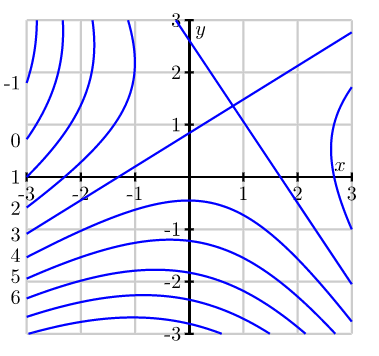
\includegraphics[scale=0.6]{contour_14_3.png}
	\end{minipage}
	

	\item The speed of sound $C$ traveling through ocean water is a function of 
	temperature, salinity, and depth.  It may be modeled by the function	
	\[C(T,S,D)=1450 +4.5T-0.05T^2+0.0003T^3+(1.5-0.01T)(S-35)+0.015D, \]
	
	where $C$ is the speed of sound in meters/second, $T$ is the temprature in degrees Celsius, $S$ is the salinity in grams/liter of water, and $D$ is the depth below the ocean surface in meters.
	
	\begin{enumerate}
		\item State the units in which each of the partial derivatives $C_T,C_S,$ and $C_D$ are expressed and explain the physical meaning of each.
		
		\item Find the partial derivatives $C_T, C_S,$ and $C_D$.
		
		\item Evaluate each of the three partial derivatives at the point where $T=10, S=35$, and $D=100$.  What does the sign of each partial derivative tell us about the behavior of the function $C$ at the point $(10,35,100)$?
	\end{enumerate}

%	\item Find $f_x$ and $f_y$ for:
%	\begin{enumerate}
%		\item $f(x,y)= x^3y^2+5y^2-x+7$
%		
%		\item $f(x,y) = e^{x^2y^3} \sqrt{x^2+1}$
%		
%		\item $f(x,y) = \cos(xy^2)+\sin(x)$
%	\end{enumerate}
	
	\item Find all the second partial derivatives for $f(x,y)=e^x+x\ln (y).$
	
	\item Find $f_x$, $f_y$, $f_z$, and $f_{xzz}$ for the function $f(x,y,z)=x\sin(yz)$.
	
	\pagebreak
	
	\item Find the total derivative $Df$ at the given point for each function below. Remember that $Df$ is the matrix of (partial) derivatives of the function and if $f$ is a function from $\R^n$ to $\R^m$ then $Df$ is a $m\times n$ matrix.
	\begin{enumerate}
		\item $f(x)=2x^3+7$ at $x=2$.
		\item $\mathbf{f}(t)=\langle 2\cos(t), 2 \sin(t), t\rangle$ at $t=\pi/2$.
		\item $f(x,y)=\sqrt{y-x}$ at $(x,y)=(1,2)$.
		\item $f(x,y,z)=e^{2y-x}+z^2+4$ at $(x,y,z)=(1,2,3)$.
		\item $\mathbf{f}(s,t) = \langle 2s+3t, t-s\rangle$ at $(s,t)=(1,1)$.  
	
		\textbf{Note:} The graph of this function is a surface (in this case all of $\R^2$) parameterized by two variables just like the graph of the function in (b) is a curve parameterized by one variable - we'll see these more later!  Another way of thinking about this is that this is a \textit{change of variables} for $\R^2$ between the system of coordinates $(s,t)$ and $(x,y)$.
	\end{enumerate}
	
	\item The fifth-order partial derivative $\partial^5f/\partial x^2\partial y^3$ is zero for each of the following functions.  To show this as quickly as possible, which variable would you differentiate with respect to first: $x$ or $y$?
	
	Try to answer without writing anything down.  Why did you make the choice you did?
	
	\begin{enumerate}
		\item $f(x,y)=y^2x^4e^x+2$
		
		\item $f(x,y)=y^2+y(\sin(x)-x^4)$
		
		\item $f(x,y)=x^2+5xy+\sin(x)+7e^x$
		
		\item $f(x,y)=xe^{y^/2}$
	\end{enumerate}
\end{enumerate}
}{}

\iftoggle{answers}{
\begin{center}{\large \textbf{Math 2551 Worksheet Answers: Partial Derivatives}}
\end{center}
\begin{enumerate}	
	\item 
	\begin{enumerate}
		\item $f_x(-2,-1)\approx 0.75$
		\item $f_y(-2,-1)\approx 1.5$
		\item There are several possible points (these are places where the tangent to a contour is horizontal): $(0,-.5),(-.5,-1.25)$, etc.
		\item Again, there are many possible points; any point on the 4, 5, 6 contours in quadrant IV will work.
	\end{enumerate}

	\item \begin{enumerate}
		\item $C_T$: (meters/second)/ degree Celsius - this gives the change in speed for each one degree C of temperature increase.
		$C_S$ (meters/second)/(grams/liter) - this gives the change in speed for each one gram/liter increase in salinity
		$C_D$: (meters/second)/meter - this gives the change in speed for each one meter increase in depth below the surface
		
		\item $C_T= 4.5-0.1T+0.0009T^2-0.01(S-35)$
		$C_S=1.5-0.01T$
		$C_D=0.015$
		
		\item At $(T,S,D)=(10,35,100)$, we have $C_T=3.59, C_S=1.4, C_D=0.015$.  This tells us that if we increase the temperature, salinity, or depth from these conditions the speed of sound will increase as well.
	\end{enumerate}
%	\item 	\begin{enumerate}
%		\item $f_x=3x^2y^2-1, f_y=2x^3y+10y$
%		
%		\item $f_x=2xy^3e^{x^2y^3}\sqrt{x^2+1}+\dfrac{x e^{x^2y^3}}{\sqrt{x^2+1}}, f_y=3x^2y^2 e^{x^2y^3}\sqrt{x^2+1}$
%		
%		\item $f_x=-y^2\sin(xy^2)+\cos(x), f_y=-2xy\sin(xy^2)$
%	\end{enumerate}
	
	\item $f_{xx}=e^x, f_{xy}=f_{yx}=\dfrac{1}{y}, f_{yy}=-\dfrac{x}{y^2}$
	
	\item $f_x=\sin(yz), f_y=xz\cos(yz), f_z=xy\cos(yz), f_{xzz}=-y^2\sin(yz)$
	
	\item Find the total derivative $Df$ at the given point for each function below. Remember that $Df$ is the matrix of (partial) derivatives of the function and if $f$ is a function from $\R^n$ to $\R^m$ then $Df$ is a $m\times n$ matrix.
	\begin{enumerate}
		\item $Df(2)=f'(2)=[24]$
		\item $D\mathbf{f}(\pi/2)=\mathbf{f}'(\pi/2)=\begin{bmatrix}
			-2 \\ 0 \\ 1
		\end{bmatrix}$
		\item $Df(1,2)=\begin{bmatrix}
			-1/2 & 1/2
		\end{bmatrix}$
		\item $Df(1,2,3)=\begin{bmatrix}
			-e^3 & 2e^3 & 6
		\end{bmatrix}$
		\item $D\mathbf{f}(1,1) = \begin{bmatrix}
			2 & 3 \\
			-1 &  1
		\end{bmatrix}  $
		
	\end{enumerate}
	\item Note this does not have a definitive right answer - some differences may arise and that's good! Discuss!
	
	\begin{enumerate}
		\item First $y$ since $\partial^3 f/\partial y^3=0$ and the $y$-partial derivatives are easier
		
		\item First $y$, since $\partial^3 f/\partial y^3=0$
		
		\item First $y$, since $\partial^2 f/\partial y^2=0$
		
		\item First $x$, since $\partial^2 f/\partial x^2=0$ and the $x$-partial derivatives are easier.
	\end{enumerate}
	
	A common theme is to work with the variable with lower powers/simpler expressions first when taking mixed partials.
	
\end{enumerate}
}{}
\iftoggle{solutions}
{
Solutions go here in the same format.
}{}
